\chapter[Momento angolare orbitale]{Momento angolare orbitale\footnote{S3.6, LL26, G11}}
Abbiamo introdotto il momento angolare definendolo come il generatore delle rotazioni infinitesime. Ma quando il momento di spin è nullo (o comunque può essere ignorato) il momento angolare per una particella coincide con il \textbf{momento angolare orbitale}, definito da:
\begin{equation}
\vec{L}=\vec{r}\wedge\vec{p}
\end{equation}
Per il momento angolare orbitale, le \textbf{regole di commutazione} fondamentali,
\begin{equation}
[L_i, L_j]= i \varepsilon _{ijk}L_k ,
\label{eq:cap17_1}
\end{equation}
seguono direttamente dalle regole di commutazione degli operatori di posizione ed impulso. Si ha, ad esempio,
\begin{eqnarray}
[L_x , L_y] &=& [y p_z - zp_y, zp_x -xp_z] = \nonumber \\
&=&[y p_z , zp_x] + [zp_y, xp_z] = \nonumber \\
&=& yp_x [p_z , z] + p_y x [z , p_z] = \nonumber  \\
&=& -i\hbar (yp_x -xp_y) = i\hbar L_z ,
\end{eqnarray}
e analoghe per le altre componenti.\\
Possiamo mostrare esplicitamente come l'operatore momento angolare, definito dall'eq. (\ref{eq:cap17_1}), coincida, per particelle di spin nullo, con il \textbf{generatore delle rotazioni infinitesime}.\\
Applichiamo infatti l'operatore:
\begin{equation}
\left(1- \frac{i}{\hbar}\delta \varphi L_z\right)
\end{equation}
su un autostato arbitrario della posizione, e mostriamo come lo stato risultante sia ancora un autostato della posizione ma ruotato, rispetto allo stato di partenza, di un angolo $\delta \varphi$ attorno all'asse $z$. Questo risultato segue dalla considerazione che l'impulso è il generatore delle traslazioni infinitesime. Si ha infatti:
\begin{eqnarray}
\left(1- \frac{i}{\hbar}\delta \varphi L_z\right)\vert x', y', z'\rangle &=& \underbrace{\left[1- \frac{i}{\hbar}\delta \varphi\left(x'p_y-y'p_x\right)\right]}_{\begin{array}{cc}
\scriptstyle{(1- \frac{i}{\hbar}\vec{p}\cdot d\vec{x})}\\
\scriptstyle{d\vec{x}= (-y\delta \varphi ,\ x \delta \varphi ,\ 0)}
\end{array}}\vert x', y', z'\rangle = \nonumber \\
&=&\vert x'-y'\delta \varphi , y'+x'\delta \varphi , z'\rangle ,
\end{eqnarray}
che è quello che volevamo dimostrare.
\begin{equation}
\textrm{N.B.} \quad 
R_z (\delta \varphi)=
\begin{pmatrix}
1 & -\delta \varphi & 0\\
\delta \varphi & 1 & 0 \\
0 & 0 & 1 \\
\end{pmatrix}
\end{equation}
Lo stesso risultato può essere convenientemente espresso utilizzando, per definire l'autostato della posizione, un sistema di coordinate polari:
\begin{equation}
\left(1- \frac{i}{\hbar}\delta \varphi L_z\right)\vert r, \theta, \varphi\rangle = \vert r, \theta, \varphi + \delta\varphi\rangle .
\label{eq:cap17_2}
\end{equation}
Proponiamoci ora di derivare l'\textbf{espressione dell'operatore $L_z$ nella rappresentazione delle coordinate}.\\
Utilizzando sempre un sistema di coordinate polari, e tenendo conto dell'eq. (\ref{eq:cap17_2}), troviamo:
\begin{eqnarray}
\langle r, \theta, \varphi \vert \left(1- \frac{i}{\hbar}\delta \varphi L_z\right) \vert \alpha\rangle &=& \langle r, \theta, \varphi \vert \left(1+ \frac{i}{\hbar}\delta \varphi L_z\right) ^+ \vert \alpha\rangle =\nonumber \\
&=& \langle r, \theta, \varphi - \delta \varphi \vert\alpha\rangle  = \nonumber \\
&=& \langle r, \theta, \varphi \vert \alpha\rangle - \delta \varphi \frac{\partial}{\partial \varphi}\langle r, \theta, \varphi \vert\alpha\rangle .
\end{eqnarray}
per l'arbitrarietà dello stato $\vert \alpha \rangle$, questo risultato implica:
\begin{equation}
\langle r, \theta, \varphi \vert  L_z \vert \alpha\rangle =- i\hbar\ \frac{\partial}{\partial \varphi}\langle r, \theta, \varphi \vert\alpha\rangle ,
\end{equation}
ossia nella rappresentazione delle coordinate
\begin{equation}
L_z = -i\hbar \frac{\partial}{\partial \varphi}.
\label{eq:cap17_4}
\end{equation}
Allo stesso stato si può giungere, altrettanto facilmente, utilizzando l'espressione nella rappresentazione delle coordinate  dell'operatore impulso. Si ha infatti:
\begin{equation}
L_z= xp_y-yp_x = -i\hbar \left( x\frac{\partial}{\partial y} -y\frac{\partial}{\partial x}\right) .
\label{eq:cap17_3}
\end{equation}
Esprimiamo questo risultato utilizzando un sistema di coordinate polari. Dalle relazioni
\begin{equation}
\begin{cases}
x=r\sin \theta \cos \varphi \\
y=r\sin \theta \sin \varphi \\
z= r\cos\theta
\end{cases}
\qquad
\begin{cases}
r=(x^2+y^2+z^2)^{1/2} \\
\theta=\arctan\left(\sqrt{(x^2+y^2)/z^2}\right) \\
\varphi= \arctan \left(y/x\right)
\end{cases}
\end{equation}
si derivano, con una semplice algebra, le relazioni\footnote{$\partial/\partial x \arctan x = 1/(1+x^2)$}
\begin{equation}
\begin{cases}
\displaystyle{\frac{\partial}{\partial x} = \frac{\partial r}{\partial x}\frac{\partial}{\partial r}+\frac{\partial \theta}{\partial x}\frac{\partial}{\partial \theta}+ \frac{\partial \varphi}{\partial x}\frac{\partial}{\partial \varphi} = }\\
\qquad = \displaystyle{\sin\theta \cos \varphi \frac{\partial}{\partial r}+\cos\theta \cos \varphi\frac{1}{r} \frac{\partial}{\partial \theta}-\frac{\sin \varphi}{r\ \sin \theta} \frac{\partial}{\partial \varphi}}; \\
\\
\displaystyle{\frac{\partial}{\partial y} = \frac{\partial r}{\partial y}\frac{\partial}{\partial r}+\frac{\partial \theta}{\partial y}\frac{\partial}{\partial \theta}+ \frac{\partial \varphi}{\partial y}\frac{\partial}{\partial \varphi} = }\\
\qquad = \displaystyle{\sin\theta \sin \varphi \frac{\partial}{\partial r}+\cos\theta \sin \varphi\frac{1}{r} \frac{\partial}{\partial \theta}+\frac{\cos \varphi}{r\ \sin \theta} \frac{\partial}{\partial \varphi}}; \\
\\
\displaystyle{\frac{\partial}{\partial z} = \frac{\partial r}{\partial z}\frac{\partial}{\partial r}+\frac{\partial \theta}{\partial z}\frac{\partial}{\partial \theta}+ \frac{\partial \varphi}{\partial z}\frac{\partial}{\partial \varphi} = }\\
\qquad = \displaystyle{\cos\theta\frac{\partial}{\partial r}-\frac{\sin \theta}{r} \frac{\partial}{\partial \theta}}.
\end{cases}
\end{equation}
Dall'espressione (\ref{eq:cap17_3}) dell'operatore $L_z$ si ottiene pertanto
\begin{eqnarray}
L_z &=&-i\hbar \left[ r\sin \theta \cos \varphi \left(\sin \theta \sin \varphi \frac{\partial}{\partial r}+\cos \theta \sin \varphi\frac{1}{r} \frac{\partial}{\partial \theta}+ \right.\right. \nonumber \\
& &\left. + \frac{\cos \varphi}{r\ \sin \theta} \frac{\partial}{\partial \varphi}\right) - r \sin \theta \sin \varphi \left( \sin \theta \cos \varphi \frac{\partial}{\partial r}+\right. \nonumber \\
& & \left. \left. \cos \theta \cos \varphi\frac{1}{r} \frac{\partial}{\partial \theta}-\frac{\sin \varphi}{r\ \sin \theta} \frac{\partial}{\partial \varphi}\right)\right] ,
\end{eqnarray}
ossia
\begin{equation}
L_z = -i\hbar \frac{\partial}{\partial \varphi},
\end{equation}
in accordo con quanto ricavato precedentemente.\\
In modo analogo si possono derivare le \textbf{espressioni degli operatori nella rappresentazione delle coordinate}. Risulta conveniente, a tale scopo, derivare prima queste espressioni per gli operatori $L_{\pm}$:
\begin{eqnarray}
L_{\pm} &=& L_x \pm iL_y = (yp_z-zp_y) \pm i(zp_x-xp_z)= \nonumber \\
&=& \mp i (x\pm iy)p_z \pm iz(p_x\pm ip_y)= \nonumber \\
&=&\mp \hbar \left[ \left(x\pm i y\right) \frac{\partial}{\partial z}- z \left( \frac{\partial}{\partial x}\pm i\frac{\partial}{\partial y}\right) \right] ,
\end{eqnarray}
da cui, sostituendo le coordinate polari:
\begin{eqnarray}
L_{\pm} &=&\mp \hbar \left[ r\sin \theta\ e^{\pm i \varphi}\ \left( \cos \theta\frac{\partial}{\partial r} -\frac{\sin \theta}{r}\frac{\partial}{\partial \theta} \right)- \right. \nonumber \\
& &\left. - r\cos \theta \left( \sin \theta\ e^{\pm i \varphi}\frac{\partial}{\partial r}+\frac{\cos \theta}{r} e^{\pm i \varphi}\frac{\partial}{\partial \theta}\pm\frac{i e^{\pm i \varphi}}{r\sin \theta}\frac{\partial}{\partial \varphi} \right)\right]= \nonumber \\
&=& \mp \hbar e^{\pm i \varphi}\left(-\frac{\partial}{\partial \theta}\mp i\ \cot \theta\frac{\partial}{\partial \varphi}\right) ,
\end{eqnarray}
ossia, infine
\begin{equation}
L_{\pm}=\hbar e^{\pm i \varphi}\left[\pm \frac{\partial}{\partial \theta}+ i\ \cot \theta\frac{\partial}{\partial \varphi}\right] .
\label{eq:cap17_5}
\end{equation}
Da questo risultato è poi immediato ricavare le espressioni degli operatori $L_x$ ed $L_y$ nella rappresentazione delle coordinate. Ricordando le relazioni:
\begin{equation}
L_x = \frac{1}{2} (L_+ + L_-) \qquad L_y = \frac{1}{2i} (L_+ + L_-),
\end{equation}
si ottiene
\begin{eqnarray}
& &L_x =i\hbar \left( \sin \varphi \frac{\partial}{\partial \theta}+\cot \theta \cos \varphi \frac{\partial}{\partial \varphi}\right)\\
& &L_y =i\hbar \left(- \cos \varphi \frac{\partial}{\partial \theta}+\cot \theta \sin \varphi \frac{\partial}{\partial \varphi}\right) .
\end{eqnarray}
Risulta infine utile determinare l'\textbf{espressione, nella rappresentazione delle coordinate, del quadrato del momento angolare orbitale}. È conveniente partire dalla relazione (refeq:cap$16_7$) che si scrive, nel caso del momento angolare orbitale,
\begin{equation}
L_- L_+ = L^2 -L_z ^2 -\hbar L_z .
\end{equation}
Ricavando $L^2$ da questa relazione e sostituendovi le espressioni (\ref{eq:cap17_4}) e (\ref{eq:cap17_5}) per $L_z$ ed $L_{\pm}$, otteniamo:
\begin{eqnarray}
L^2 &=& L_-L_+ L_z^2 +\hbar L_z = \nonumber \\
&=& \hbar ^2 \left[e^{-i\varphi}\ \left(-\frac{\partial}{\partial \theta}+i \cot \theta\ \frac{\partial}{\partial \varphi}\right)e^{i\varphi}\ \left(\frac{\partial}{\partial \theta}+i \cot \theta\ \frac{\partial}{\partial \varphi}\right)-\right. \nonumber \\
& &\qquad \left. -\frac{\partial ^2}{\partial \varphi ^2}- i\frac{\partial}{\partial \varphi}\right] = \nonumber \\
&=&\hbar ^ 2 \left[ \left( -\frac{\partial}{\partial \theta}-\cot\theta +i \cot\theta\ \frac{\partial}{\partial \varphi}\right)\left(\frac{\partial}{\partial \theta}+i \cot \theta \ \frac{\partial}{\partial \varphi}\right)-\right. \nonumber \\
& &\qquad \left. -\frac{\partial ^2}{\partial \varphi ^2}- i\frac{\partial}{\partial \varphi}\right] = \nonumber \\
&=& \hbar ^2 \left[ -\frac{\partial ^2}{\partial \theta ^2}-i\left( \frac{\partial \cot \theta}{\partial \theta}\right) \frac{\partial }{\partial \varphi }-i\cot \theta \frac{\partial ^2}{\partial \theta \partial \varphi}-\cot \theta\ \frac{\partial }{\partial \theta}-\right. \nonumber \\
& & \left. -i \cot ^2 \theta \frac{\partial }{\partial \varphi}+i \cot\theta \frac{\partial ^2}{\partial \theta \partial \varphi}-\cot ^2 \theta \frac{\partial ^2}{\partial \varphi ^2}-\frac{\partial ^2}{\partial \varphi ^2}-i\frac{\partial }{\partial \varphi}\right] = \nonumber \\
&=& \hbar^2 \left[ -\frac{\partial ^2}{\partial \theta ^2}-\cot \theta \frac{\partial }{\partial \theta}-\left(1+ \cot ^2 \theta\right) \frac{\partial ^2}{\partial \varphi ^2}+\right. \nonumber \\
& &\qquad \left. -i\left( 1+\cot ^2 \theta +\frac{\partial \cot \theta}{\partial \theta}\right)\frac{\partial}{\partial \varphi}\right] .
\end{eqnarray}
Considerando le relazioni
\begin{equation}
1+ \cot ^2 \theta = 1+\frac{\cos ^2 \theta}{\sin ^2 \theta} = \frac{1}{\sin ^2 \theta},
\end{equation}
\begin{equation}
\frac{\partial \cot \theta}{\partial \theta}= \frac{\partial}{\partial \theta}\left( \frac{\cos  \theta}{\sin \theta} \right) = \frac{-\sin ^ 2 \theta - \cos ^2 \theta}{\sin ^2 \theta}=-\frac{1}{\sin ^2 \theta},
\end{equation}
possiamo scrivere
\begin{equation}
L^2 = \hbar ^2 \left[- \frac{\partial ^2}{\partial \theta ^2}-\cot \theta \frac{\partial}{\partial \theta}- \frac{1}{\sin ^2 \theta}\frac{\partial ^2}{\partial \varphi ^2}\right] ,
\end{equation}
o, equivalentemente:
\begin{equation}
L^2 = -\hbar ^2 \left[\frac{1}{\sin ^2 \theta}\frac{\partial ^2}{\partial \varphi ^2}+\frac{1}{\sin \theta}\frac{\partial}{\partial \theta} \left(\sin \theta \frac{\partial}{\partial \theta}\right)\right] .
\end{equation}
Osserviamo che, a meno di un fattore, $L^2$ è la parte angolare dell'operatore di Laplace.
\section[Autovalori del momento angolare orbitale e armoniche sferiche]{Autovalori del momento angolare orbitale e armoniche sferiche\footnote{S3.6, LL27-28, G11}}
Consideriamo gli autostati simultanei degli operatori $L^2$ ed $L_z$, definiti dalle equazioni:
\begin{eqnarray}
& &L^2 \vert l, m \rangle = \hbar ^2 l(l+1) \vert l, m \rangle ,\label{eq:cap17_6}\\
& &L_z \vert l, m \rangle = \hbar m \vert l, m \rangle \label{eq:cap17_7}.
\end{eqnarray}
Seguendo una pratica usuale abbiamo qui indicato con $l$ il numero quantico $j$ riferito al momento angolare orbitale. La componente $z$ del momento angolare può quindi assumere i valori definiti da
\begin{equation}
m = -l, -l+1, \dots,l-1, l .
\end{equation}
\textbf{L'assegnazione dei valori $l$ ed $m$ non definisce completamente lo stato della particella}. Ciò è evidente già dal fatto che le espressioni degli operatori $L^2$ e $L_z$, in coordinate sferiche, contengono solamente gli angoli $\theta$ e $\varphi$, così che le loro autofunzioni possono contenere un fattore arbitrario dipendente da $r$- In questo contesto ci limitiamo allora solo a considerare la parte dipendente dagli angoli $\theta$ e $\varphi$ degli autostati di posizione; in altri termini, indicheremo con $\vert \theta ,\varphi\rangle$ il vettore di stato di una particella che si trova in un punto dello spazio individuato dagli angoli $\theta $ e $\varphi$, ma a distanza $r$ arbitraria dall'origine delle coordinate.\\
Moltiplichiamo scalarmente entrambi i membri delle equazioni (\ref{eq:cap17_6}) e (\ref{eq:cap17_7}) per il bra $\langle \theta , \varphi \vert$:
\begin{eqnarray}
& &\langle \theta , \varphi \vert L^2 \vert l, m \rangle = \hbar ^2 l(l+1) \langle \theta , \varphi \vert l, m \rangle ,\\
& &\langle \theta , \varphi \vert L_z \vert l, m \rangle = \hbar m\langle \theta , \varphi \vert l, m \rangle .
\end{eqnarray}
Le funzioni
\begin{equation}
Y_{l,m} (\theta, \varphi )= \langle \theta , \varphi \vert l, m \rangle 
\end{equation}
sono dunque le \textbf{autofunzioni simultanee degli operatori $L^2$ ed $L_z$} e sono note con il nome di \textbf{armoniche sferiche}. Fisicamente, queste funzioni rappresentano l'\textbf{ampiezza di probabilità che un sistema, caratterizzato dai valori $l$ ed $m$ dei numeri quantici del momento angolare, si trovi in una posizione la cui direzione è definita dal valori $\theta$ e $\varphi$ degli angoli delle coordinate polari}.\\
Le espressioni derivate in precedenza per gli operatori del momento angolare nella rappresentazione delle coordinate, ci consentono di scrivere esplicitamente le \textbf{equazioni agli autovalori che definiscono le armoniche sferiche}:
\begin{eqnarray}
L^2 Y_{l,m} (\theta, \varphi) &=&-\hbar ^2 \left[\frac{1}{\sin ^2 \theta}\frac{\partial ^2}{\partial \varphi ^2}+\frac{1}{\sin \theta}\frac{\partial}{\partial \theta} \left(\sin \theta \frac{\partial}{\partial \theta}\right)\right]Y_{l,m}(\theta, \varphi) = \nonumber \\
&=& \hbar ^2 l(l+1)Y_{l,m}(\theta, \varphi) ,\label{eq:cap17_8}\\
& &\nonumber \\
L_zY_{l,m}(\theta, \varphi)&=& -i\hbar \frac{\partial}{\partial \varphi}Y_{l,m}(\theta, \varphi)= \hbar m Y_{l,m}(\theta, \varphi) \label{eq:cap17_9}.
\end{eqnarray}
Dalla condizione di normalizzazione degli autostati $\vert l,m \rangle$ e dalla completezza degli autostati $\vert \theta , \varphi\rangle $ della posizione, segue la condizione di normalizzazione delle armoniche sferiche:
\begin{equation}
\langle l' , m' \vert l,m \rangle = \int d\Omega \ \langle l' ,m'\vert \theta, \varphi \rangle \langle \theta , \varphi \vert l, m \rangle = \delta _{ll'} \delta _{mm'} ,
\end{equation}
ossia
\begin{equation}
\int _0 ^{2\pi} d\varphi \int _{-1} ^1 d(\cos \theta )\ Y_{l',m'}^* (\theta , \varphi ) Y_{l,m} (\theta, \varphi )=\delta _{ll'} \delta _{mm'}.
\end{equation}
Le equazioni differenziali (\ref{eq:cap17_8}) e (\ref{eq:cap17_9}), che definiscono le armoniche sferiche, ammettono una soluzione per separazione delle variabili $\theta$ e $\varphi)$, della forma:
\begin{equation}
Y_{l,m} (\theta , \varphi ) = \Theta _{l,m}(\theta)\Phi _m (\varphi) ,
\end{equation} $\Theta _{l,m}(\theta)$ e $\Phi _m (\varphi)$ sono separatamente normalizzate:
\begin{eqnarray}
& & \int d\varphi\ \vert \Phi _m (\varphi)\vert ^2 =1, \nonumber\\
\\
& & \int d\varphi\ \vert \Theta _{l,m}(\theta) \vert ^2 =1. \nonumber
\end{eqnarray}
L'eq. (\ref{eq:cap17_9}) indica che le funzioni $\Phi _m$ sono in particolare le autofunzioni della componente $z$ del momento angolare, mentre le funzioni $\Theta _{l,m}$ non sono di per sé autofunzioni di qualche operatore del momento angolare.\\
L'eq. (\ref{eq:cap17_9}), che possiamo scrivere nella forma:
\begin{equation}
-i\frac{\partial}{\partial \varphi}\Phi _m (\varphi )= m \Phi _m (\varphi ) ,
\end{equation}
ha come soluzioni normalizzate le funzioni:
\begin{equation}
\Phi _m (\varphi ) = \frac{1}{\sqrt{2\pi}}e^{im\varphi} .
\end{equation}
La condizione che la funzione d'onda sia monotona (ossia ad un solo valore) implica in particolare
\begin{equation}
\Phi _m (0) =\Phi _m (2\pi ) ,
\label{eq:cap17_10}
\end{equation}
e dunque \textbf{l'autovalore $m$ può assumere solo valori interi} (positivi o negativi):
\begin{equation}
m= 0, \pm 1,\pm 2, \dots
\end{equation}
ne segue che anche \textbf{il numero $l$ può assumere solo valori interi} (positivi, incluso lo zero):
\begin{equation}
l= 0,1,2,\dots
\end{equation}
\textbf{Sottolineiamo come le regole di commutazione del momento angolare implichino soltanto la condizione che $j$ (o $l$) e, dunque, $m$  siano numeri intero o semi-interi. La condizione che $l$ ed $m$ siano invece numeri interi è una condizione aggiunta valida specificatamente per il momento angolare orbitale e che non si applica pertanto al momento angolare di spin}.\\
La determinazione delle funzioni $\Theta _{lm} (\theta)$ può essere effettuata risolvendo l'equazione agli autovalori per l'operatore $L^2$ e sostituendo per $\Phi _m (\varphi)$ la sua espressione (\ref{eq:cap17_10}). Risulta tuttavia conveniente seguire un'altra strada\footnote{Il procedimento qui esposto è il cosiddetto metodo matriciale, analogo a quello discusso per le autofunzioni dell'oscillatore atmonico.}. Consideriamo in primo luogo l'autostato corrispondente ad $m=l$. Questo soddisfa l'equazione
\begin{equation}
L_+ \vert l,l\rangle =0,
\end{equation}
la cui espressione, nella rappresentazione delle coordinate si ottiene moltiplicando l'equazione per il bra $\vert \theta, \varphi \rangle$ ed utilizzando per  l'operatore $L_+$ la sua rappresentazione(\ref{eq:cap17_5}). Si ottiene in tal modo:
\begin{equation}
L_+Y_{ll}(\theta , \varphi ) = \hbar e^{i\varphi}\left[\frac{\partial}{\partial\theta}+i \cot\theta \frac{\partial}{\partial \varphi}\right]Y_{ll}(\theta , \varphi ) =0 .
\end{equation}
Sostituendo nella precedente equazione 
\begin{equation}
Y_{ll}(\theta , \varphi ) = \frac{1}{\sqrt{2\pi}}e^{il\varphi}\ \Theta _{ll} (\theta ) ,
\end{equation}
Otteniamo per $\Theta _{ll} (\theta )$ l'equazione
\begin{equation}
\frac{d\Theta _{ll}}{d \theta}-l\cot\theta \ \Theta _{ll} (\theta )=0 ,
\end{equation}
la cui soluzione si ricava facilmente
\begin{eqnarray}
& &\frac{d\Theta _{ll}}{d \theta}=l\cot\theta \ \Theta _{ll} (\theta ) \Rightarrow \nonumber \\
& &\Rightarrow \ln \Theta _{ll} = l \int d\theta \ \frac{\cos \theta}{\sin \theta}+ \textrm{cost} = l \int  \frac{d\sin \theta}{\sin \theta}+ \textrm{cost} \nonumber \\
& & \qquad \qquad = l \log \sin \theta + \textrm{cost} ,
\end{eqnarray}
ossia
\begin{equation}
\Theta _{ll} (\theta )= c_l \sin ^l \theta .
\end{equation}
la costante $c_l$ si ricava (a meno di una fase arbitraria) dalla condizione di normalizzazione:
\begin{equation}
\int _{-1} ^1 d(\cos \theta )\ \vert \Theta _{ll} (\theta ) \vert ^2 = \vert c_l \vert ^2 \int _{-1} ^1 d(\cos \theta )\ \left( \sin \theta \right) ^{2l} =1.
\end{equation}
Per determinare il valore dell'integrale effettuiamo in primo luogo un'integrazione per parti:
\begin{eqnarray}
\int _{-1} ^1 d(\cos \theta )\ (\sin \theta ) ^{2l} &=& \int _{0} ^{\pi} d\theta \sin \theta\ (\sin \theta ) ^{2l} = \nonumber \\
&=& \left. -\cos \theta (\sin \theta ) ^{2l} \right\vert _0 ^{\pi} +2l\int _{0} ^{\pi} d\theta \cos ^2 \theta \ (\sin \theta ) ^{2l-1} = \nonumber \\
&=&  2l\int _{0} ^{\pi} d\theta \ (\sin \theta ) ^{2l-1} - 2l\int _{0} ^{\pi} d\theta  \ (\sin \theta ) ^{2l+1} .
\end{eqnarray}
Vediamo allora che 
\begin{equation}
\int _{0} ^{\pi} d\theta \ (\sin \theta ) ^{2l+1}=\frac{2l}{2l+1} \int _{0} ^{\pi} d\theta \ (\sin \theta ) ^{2l-1}.
\end{equation}
Applicando ricorsivamente questa formula otteniamo:
\begin{eqnarray}
\int _{0} ^{\pi} d\theta \ (\sin \theta ) ^{2l+1} & = & \frac{2l(2l-2)}{(2l+1)(2l-1)} \int _{0} ^{\pi} d\theta \ (\sin \theta ) ^{2l-3} = \nonumber \\
&=& \frac{2l(2l-2)\dots 2}{(2l+1)(2l-1)\dots 3} \int _{0} ^{\pi} d\theta \ \sin \theta =\nonumber \\
&=& \frac{[2l(2l-2)\dots 2]^2}{(2l+1)(2l-1)\dots 2\cdot 1}\cdot 2 \nonumber \\
& = &  \frac{[2^l\ l(l-1)(l-2)\dots 1]^2}{(2l+1)!}\cdot 2 \nonumber \\
&=& \frac{2[2^l\ l!]^2}{(2l+1)!}.
\end{eqnarray}
L'inverso di questo integrale è pari a $\vert c_l \vert ^2$. La fase di $c_l$ è scelta per convenzione uguale a $(-1)^l$, così che in definitiva si ottiene
\begin{equation}
\Theta _{ll} (\theta ) = (-1)^l \sqrt{\frac{(2l+1)!}{2}}\frac{1}{2^l\ l!}\sin^l \theta ,
\end{equation}
e per l'autofunzione completa l'espressione
\begin{equation}
Y_{ll} (\theta , \varphi) = (-1)^l \sqrt{\frac{(2l+1)!}{4\pi}}\frac{1}{2^l\ l!}e^{il\varphi} \sin ^l \theta  .
\end{equation}
Le autofunzioni $Y_{lm}(\theta , \varphi)$ con $m<l$ possono essere determinate mediante successive applicazione dell'operatore a scala $L_-$. Dalla relazione
\begin{eqnarray}
L_-\vert l, m+1 \rangle &=& \hbar \sqrt{l(l+1) - m(m+1)} \vert l,m \rangle = \nonumber \\
&=& \hbar \sqrt{(l-m)(l+m+1)} \vert l,m \rangle ,
\end{eqnarray}
vediamo che 
\begin{equation}
(L_-)^2 \vert l, m+2 \rangle = \hbar ^2 \sqrt{(l-m)(l-m-1)(l+m+1)(l+m+2)}\vert l,m \rangle ,
\end{equation}
e dunque
\begin{equation}
(L_-)^{l-m} \vert l, l \rangle = \hbar ^{l-m} \sqrt{\frac{(l-m)!(2l)!}{(l+m)!}}\vert l,m \rangle .
\end{equation}
Moltiplicando scalarmente questa relazione per il bra $\langle \theta , \varphi \vert $ otteniamo per le autofunzioni del momento angolare
\begin{equation}
Y_{lm} (\theta ,  \varphi ) = \frac{(L_-)^{l-m}}{(\hbar )^{l-m}}\sqrt{\frac{(l+m)!}{(l-m)!(2l)!}} Y_{ll} (\theta , \varphi) . 
\end{equation}
Questa formula, insieme all'espressione (\ref{eq:cap17_5}) dell'operatore $L_-$ nella rappresentazione delle coordinate, risolve completamente il problema posto.\\
È anche possibile derivare una formula esplicita per l'applicazione successiva dell'operatore $L_-$. Secondo questa formula:
\begin{equation}
\frac{1}{(\hbar) ^{l-m}}(L_-)^{l-m} \left( e^{il\varphi} f(\theta) \right) = \frac{e^{im\varphi}}{(\sin \theta ) ^m} \frac{d^{l-m}}{(d\cos \theta )^{l-m}}\left( \sin ^l \theta \ f(\theta ) \right).
\end{equation}
Utilizzando questo risultato si ottiene allora:
\begin{equation}
Y_{lm} (\theta ,  \varphi ) = \frac{(-1)^{l}}{2^l\ l!}\sqrt{\frac{(2l+1)}{4\pi}\frac{(l+m)!}{(l-m)!}}  \frac{e^{im\varphi}}{(\sin \theta ) ^m} \frac{d^{l-m}}{(d\cos \theta )^{l-m}}\left( \sin  \theta \right) ^{2l}.
\end{equation}
la dipendenza dall'angolo $\theta$ delle funzioni armoniche sferiche è rappresentata da una classe speciale di polinomi in $\cos \theta$, detti \textbf{polinomi associati di Legendre}, indicati solitamente con il simbolo $P_l ^m (\cos \theta)$. In particolare, per i valori di $m$ positivi si ha 
\begin{equation}
Y_{lm} (\theta ,  \varphi ) = \sqrt{\frac{(2l+1)}{4\pi}\frac{(l+m)!}{(l-m)!}}\ P_l ^m (\cos \theta)\ e^{im\varphi}\qquad m>0.
\end{equation}
Le armoniche sferiche con valori negativi di $m$ si possono poi scrivere, in termini delle armoniche sferiche con $m$ positivo, nella forma
\begin{equation}
Y_{lm} (\theta ,  \varphi ) = (-1)^{|m|}\left(Y_{l|m|} (\theta ,  \varphi )\right) ^* \qquad m<0.
\end{equation}
\newpage
\begin{figure}[!htbp]
\begin{center}
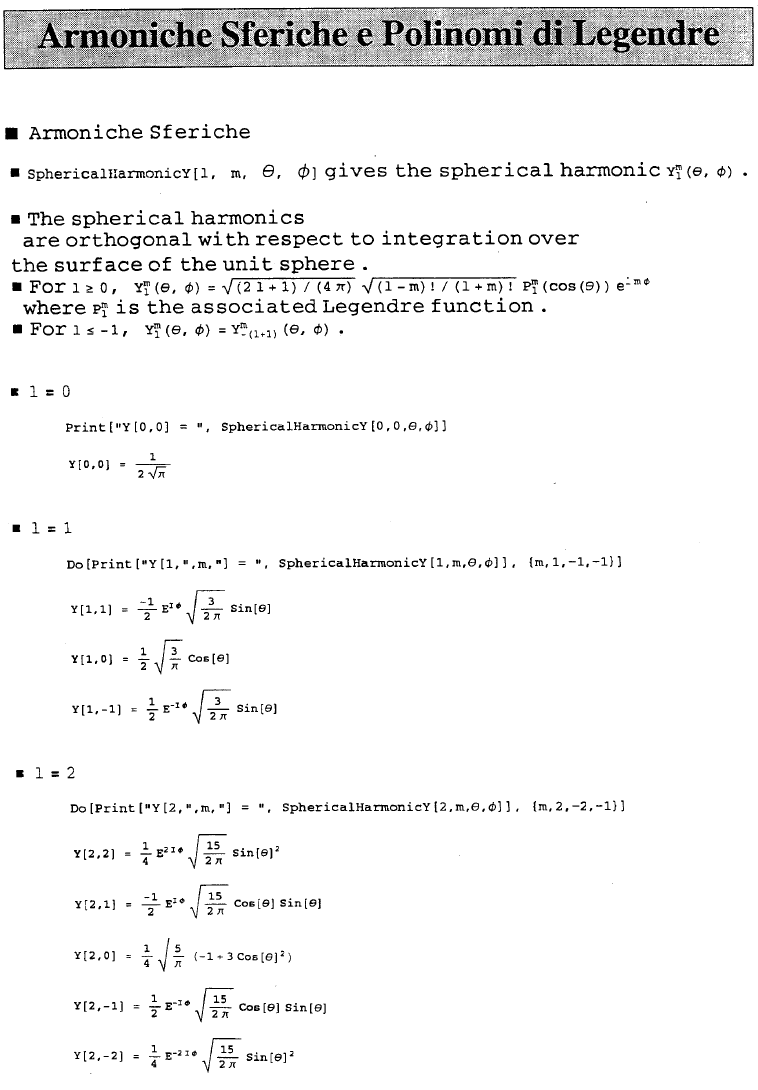
\includegraphics[width=\textwidth]{immagini/cap_17/fig_17_1.png}\\
\end{center}
\end{figure}
\begin{figure}[!htbp]
\begin{center}
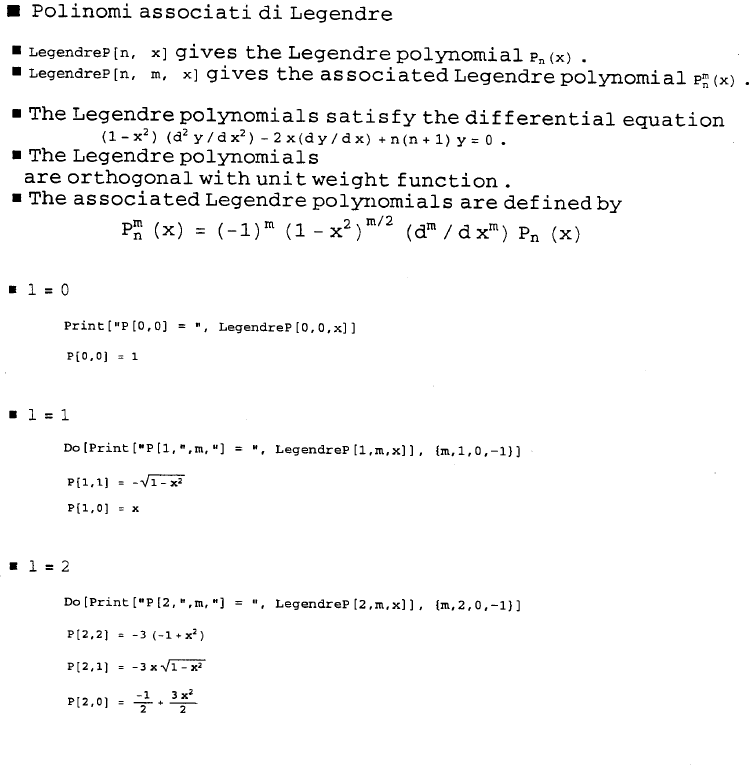
\includegraphics[width=\textwidth]{immagini/cap_17/fig_17_2.png}\\
\end{center}
\end{figure}
